%============================================================
%  Capitolo 16 – Flow Matching e Stable Diffusion 3
%============================================================
\chapter{Flow Matching e Stable Diffusion 3}
\label{ch:flow-matching}

Il \textbf{Flow Matching} (FM) è un paradigma per l'addestramento di
modelli generativi basati su flussi continui normalizzanti (\emph{Continuous
Normalizing Flows}, CNF). Rispetto ai modelli di diffusione classici,
il Flow Matching offre un approccio \emph{simulation-free}: non è
necessario simulare la traiettoria stocastica durante il training, ma
si specifica direttamente il campo vettoriale desiderato e si ottimizzano
i parametri per approssimarlo \citep{lipman2022flow,bishop2024}.

%------------------------------------------------------------
\section{Il Problema della Modellazione Generativa}
\label{sec:fm-generative-problem}

Il problema fondamentale della modellazione generativa consiste nel trovare
una trasformazione $\Phi$ che mappi campioni provenienti da una distribuzione
sorgente $p$ (tipicamente un rumore gaussiano semplice) verso la distribuzione
target $q$ dei dati reali:
\begin{equation}
  X_1 = \Phi(X_0), \qquad X_0 \sim p,\quad X_1 \sim q.
  \label{eq:fm-gen-problem}
\end{equation}
In $\mathbb{R}^d$, ogni immagine (o dato) è un punto, e le distribuzioni
$p$ e $q$ sono insiemi di concentrazione di massa probabilistica nella
stessa spazio ad alta dimensione. Il modello deve imparare a trasportare
la massa da $p$ a $q$.

\subsection{Mappatura Diretta}
\label{subsec:fm-direct-mapping}

L'approccio più immediato è apprendere direttamente la funzione
$X_1 = \Phi(X_0)$ con una rete neurale. Questa strategia ha come
pregio la semplicità e il \textbf{campionamento efficiente} (un solo
forward pass), ma presenta due limiti fondamentali:

\begin{itemize}
  \item Non è intrinsecamente \textbf{probabilistica}: non modella
        esplicitamente la densità della distribuzione target.
  \item Richiede una funzione di perdita \textbf{min-max}, tipicamente
        avversariale (GAN), che è notoriamente instabile durante l'addestramento.
\end{itemize}

\subsection{Processi di Markov a Tempo Continuo}
\label{subsec:fm-ctmp}

Una soluzione più ricca consiste nel modellare la trasformazione come
un \textbf{processo stocastico a tempo continuo} $(X_t)_{0 \le t \le 1}$:
\begin{equation}
  X_{t+h} \leftarrow \Phi_{t+h \mid t}(X_t).
\end{equation}
A seconda della natura dell'operatore di transizione $\Phi_{t+h \mid t}$,
si distinguono tre famiglie principali di processi:

\begin{description}
  \item[\textbf{Flow}] Traiettorie lisce e deterministiche; $\Phi$ è un
        diffeomorfismo.
  \item[\textbf{Diffusione}] Traiettorie stocastiche governate da un'equazione
        differenziale stocastica (SDE); spazio di design più ampio ma
        campionamento più lento.
  \item[\textbf{Jump}] Processi con discontinuità finite; raramente usati
        per dati continui come immagini.
\end{description}

Il \emph{percorso di probabilità marginale} $p_t$ descrive come la
distribuzione marginale dei campioni si trasforma nel tempo:
$X_t \sim p_t$, con $p_0 = p$ e $p_1 = q$.

\begin{figure}[H]
  \centering
  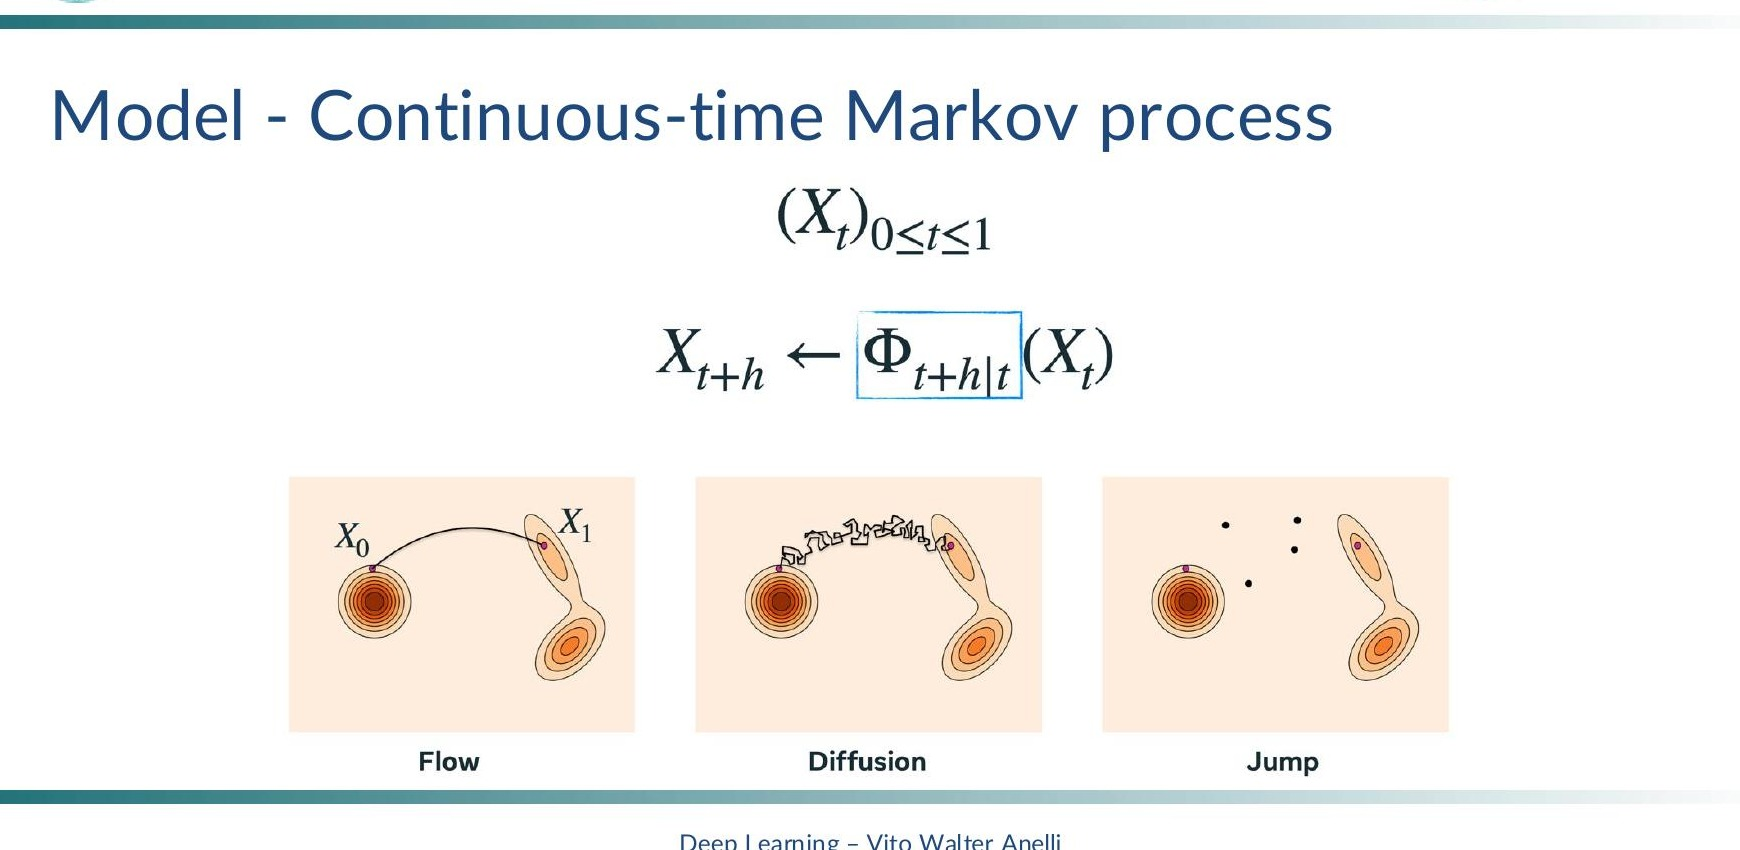
\includegraphics[width=0.82\linewidth]{figures/cf16_ctmp_types.jpg}
  \caption{Le tre famiglie di processi di Markov a tempo continuo.
           \textbf{Flow}: traiettoria liscia e deterministica dal rumore
           al dato. \textbf{Diffusione}: percorso stocastico con
           fluttuazioni browniane. \textbf{Jump}: transizioni discrete
           nello spazio.}
  \label{fig:fm-ctmp-types}
\end{figure}

\subsection{Vantaggi dei Flussi Rispetto alla Diffusione}
\label{subsec:fm-flow-advantages}

I modelli basati su flussi deterministici presentano vantaggi operativi
significativi rispetto ai modelli di diffusione stocastici:

\begin{itemize}
  \item \textbf{Semplicità}: le traiettorie sono lisce e non presentano
        fluttuazioni stocastiche.
  \item \textbf{Campionamento rapido}: è sufficiente risolvere una sola
        ODE, con minor numero di step rispetto alle SDE.
  \item \textbf{Stima esatta della verosimiglianza}: tramite il
        \emph{teorema di cambiamento di variabile} per i flussi continui,
        la log-likelihood è calcolabile in forma chiusa.
  \item \textbf{Flessibilità}: la struttura del flusso è facilmente
        componibile e modificabile.
\end{itemize}

I modelli di diffusione, pur avendo uno spazio di design più ampio,
richiedono in genere la stima di un lower bound (ELBO) della
log-likelihood e un campionamento più lento \citep{ho2020ddpm,bishop2024}.

%------------------------------------------------------------
\section{Flussi, Campi Vettoriali e Velocità}
\label{sec:fm-flows-velocity}

\subsection{Relazione tra Flusso e Campo Vettoriale}
\label{subsec:fm-flow-vector-field}

Un \textbf{campo vettoriale} su $\mathbb{R}^d$ è una funzione
$f : \mathbb{R}^d \to \mathbb{R}^d$ che assegna a ogni punto $x$ dello
\emph{spazio delle fasi} un vettore $v = \dot{x}(t)$. Il
\textbf{campo vettoriale associato al flusso} $\phi_t$ è definito come:
\begin{equation}
  f(x) = \frac{d}{dt}\phi_t(x)\bigg|_{t=0}.
\end{equation}
Poiché $\phi_t(x_0) = x(t)$, il flusso $\phi_t(x)$ è la soluzione al
\textbf{problema ai valori iniziali}:
\begin{equation}
  \frac{d}{dt}\phi_t(x_0) = f\bigl(\phi_t(x_0)\bigr), \qquad \phi_0(x_0) = x_0.
\end{equation}

\subsection{Il Flusso come Funzione di Warping}
\label{subsec:fm-flow-warping}

Un modello generativo basato su flusso apprende una funzione di warping
$\psi_t : \mathbb{R}^d \to \mathbb{R}^d$ parametrizzata da $t \in [0,1]$:
\begin{equation}
  X_t = \psi_t(X_0), \qquad X_0 \sim p, \quad t \in [0,1].
\end{equation}
Il flusso è equivalente, in forma Markoviana, all'aggiornamento:
\begin{equation}
  X_{t+h} = \psi_{t+h \mid t}(X_t).
\end{equation}

La relazione fondamentale tra il flusso $\psi_t$ e la \textbf{velocità}
$u_t$ è data dall'ODE:
\begin{equation}
  \frac{d}{dt}\psi_t(x) = u_t\bigl(\psi_t(x)\bigr).
  \label{eq:fm-ode}
\end{equation}
Dato il flusso, si può ricavare la velocità per differenziazione;
dato il campo di velocità, si può ricavare il flusso integrando l'ODE.

\subsection{Velocità e Distribuzione Marginale}
\label{subsec:fm-velocity-marginal}

Si dice che la velocità $u_t$ \textbf{genera} la distribuzione marginale
$p_t$ se, partendo da campioni $X_0 \sim p$, il processo
$X_t = \psi_t(X_0) \sim p_t$ per ogni $t \in [0,1]$.

\begin{itemize}
  \item \textbf{Pro}: la parametrizzazione tramite velocità è lineare
        rispetto al campo vettoriale (facilita l'apprendimento).
  \item \textbf{Contro}: per generare nuovi campioni è necessario
        simulare (integrare) l'ODE, il che richiede un solutore numerico.
\end{itemize}

\begin{figure}[H]
  \centering
  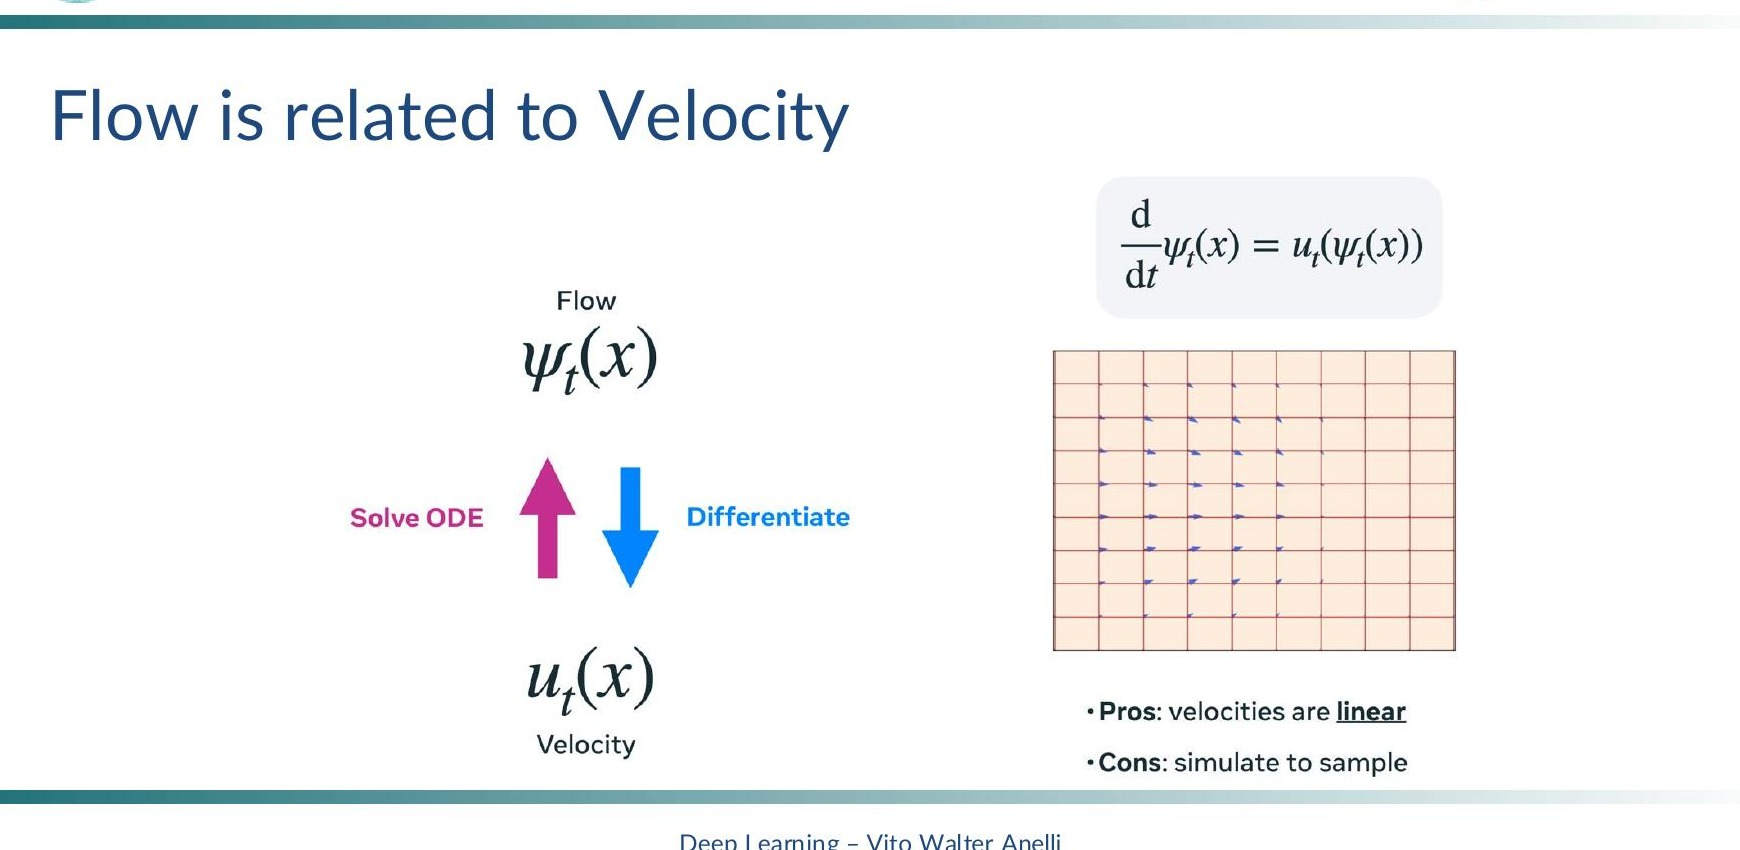
\includegraphics[width=0.72\linewidth]{figures/cf16_velocity_field.jpg}
  \caption{Rappresentazione del campo di velocità $u_t(x)$ su una griglia.
           Ogni freccia indica la direzione e l'intensità dello spostamento
           per i campioni che passano per quella posizione al tempo $t$.}
  \label{fig:fm-velocity-field}
\end{figure}

%------------------------------------------------------------
\section{L'Obiettivo di Flow Matching}
\label{sec:fm-objective}

\subsection{Formulazione Generale}
\label{subsec:fm-general-formulation}

L'idea chiave del Flow Matching è di apprendere una rete neurale
$u_t^\theta : [0,1] \times \mathbb{R}^d \to \mathbb{R}^d$ che approssimi
il campo di velocità marginale $u_t$ capace di trasportare $p_0 = p$ in
$p_1 = q$. Il processo si articola in due fasi:

\begin{enumerate}
  \item \textbf{Training}: minimizzare una funzione di perdita che misura
        la discrepanza tra $u_t^\theta$ e il campo di velocità target.
  \item \textbf{Campionamento}: partire da $X_0 \sim p$ e integrare l'ODE
        $\frac{d}{dt}X_t = u_t^\theta(X_t)$ con un solutore numerico
        (es.\ metodo del punto medio), ottenendo $X_1 \sim q$.
\end{enumerate}

\begin{figure}[H]
  \centering
  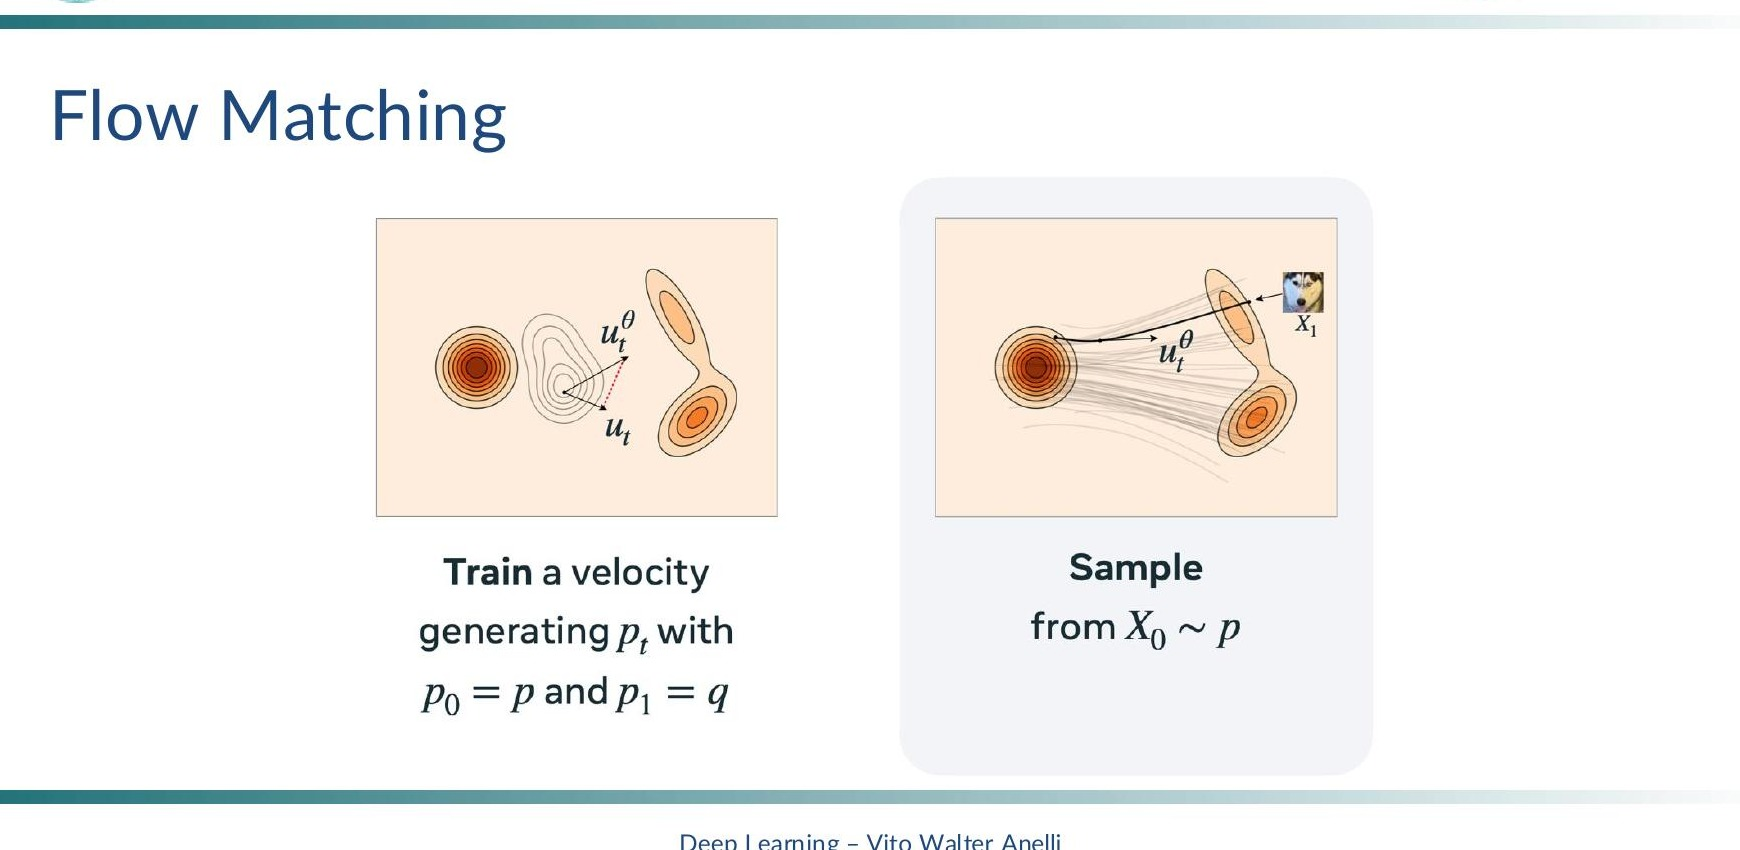
\includegraphics[width=0.85\linewidth]{figures/cf16_fm_train_sample.jpg}
  \caption{Schema di Flow Matching. \textbf{Sinistra}: durante il training,
           la rete $u_t^\theta$ (freccia rossa) viene allineata al campo
           di velocità target $u_t$ (freccia nera). \textbf{Destra}:
           durante il campionamento, le traiettorie sono integrate seguendo
           $u_t^\theta$ a partire da rumore gaussiano $X_0 \sim p$.}
  \label{fig:fm-train-sample}
\end{figure}

\subsection{Versione Più Semplice di Flow Matching}
\label{subsec:fm-simplest-version}

La versione più semplice e pratica del Flow Matching si ottiene
interpolando linearmente tra rumore e dato:
\begin{equation}
  X_t = (1-t)\,X_0 + t\,X_1, \qquad X_0 \sim p,\; X_1 \sim q,
  \label{eq:fm-linear-interp}
\end{equation}
con velocità condizionale costante $u_t(X_t \mid X_1) = X_1 - X_0$.
La funzione di perdita è:
\begin{equation}
  \mathcal{L}(\theta) = \mathbb{E}_{t,\,X_0,\,X_1}\left\|
    u_t^\theta(X_t) - (X_1 - X_0)
  \right\|^2.
  \label{eq:fm-simple-loss}
\end{equation}
In codice PyTorch, il training loop corrispondente è:
\begin{verbatim}
for _ in range(10000):
    x_1 = Tensor(make_moons(256, noise=0.05)[0])
    x_0 = torch.randn_like(x_1)
    t   = torch.rand(len(x_1), 1)
    x_t = (1 - t) * x_0 + t * x_1
    dx_t = x_1 - x_0
    optimizer.zero_grad()
    loss_fn(flow(x_t, t), dx_t).backward()
    optimizer.step()
\end{verbatim}

Il motivo per cui questo funziona risiede nella struttura teorica del
\textbf{Conditional Flow Matching}: il flusso marginale viene costruito
per sovrapposizione di flussi condizionali elementari, ognuno relativo
a un singolo punto target $x_1$.

%------------------------------------------------------------
\section{Flussi Condizionali e il Trucco della Marginalizzazione}
\label{sec:fm-conditional-flows}

\subsection{Costruzione del Flusso da Flussi Condizionali}
\label{subsec:fm-conditional-construction}

Per un singolo punto target $x_1$, si definisce il \textbf{flusso
condizionale}:
\begin{equation}
  X_t = \psi_t(X_0 \mid x_1) = (1-t)\,X_0 + t\,x_1,
\end{equation}
con distribuzione condizionale $p_{t|1}(x \mid x_1)$ e velocità
condizionale $u_t(x \mid x_1)$.

Il flusso e la velocità \textbf{marginali} si ottengono mediando
rispetto alla distribuzione dei dati $q(x_1)$:
\begin{align}
  p_t(x) &= \mathbb{E}_{X_1}\!\left[p_{t|1}(x \mid X_1)\right], \\
  u_t(x) &= \mathbb{E}\!\left[u_t(X_t \mid X_1)\,\Big|\, X_t = x\right].
\end{align}

\subsection{Teorema di Marginalizzazione}
\label{subsec:fm-marginalization-trick}

\begin{theorem}[Marginalizzazione]
La velocità marginale $u_t$ genera il percorso di probabilità marginale
$p_t$. In particolare:
\begin{equation}
  u_t(x) = \mathbb{E}\!\left[u_t(X_t \mid X_1)\,\big|\, X_t = x\right],
  \qquad
  p_t(x) = \mathbb{E}_{X_1}\!\left[p_{t|1}(x \mid X_1)\right].
\end{equation}
\end{theorem}

Questo teorema garantisce che minimizzare la perdita condizionale
\eqref{eq:cfm-loss} sia equivalente a minimizzare la perdita marginale
\eqref{eq:fm-loss}, poiché i loro gradienti rispetto a $\theta$
coincidono.

%------------------------------------------------------------
\section{Funzioni di Perdita per Flow Matching}
\label{sec:fm-losses}

\subsection{Perdita FM e Perdita CFM}
\label{subsec:fm-cfm-losses}

La \textbf{Flow Matching loss} (FM) è:
\begin{equation}
  \mathcal{L}_{\mathrm{FM}}(\theta) =
  \mathbb{E}_{t,\,X_t}\left\|u_t^\theta(X_t) - u_t(X_t)\right\|^2,
  \label{eq:fm-loss}
\end{equation}
dove $u_t$ è il campo di velocità marginale (non direttamente accessibile
in pratica, poiché richiede di conoscere $q$ in forma chiusa).

La \textbf{Conditional Flow Matching loss} (CFM) è:
\begin{equation}
  \mathcal{L}_{\mathrm{CFM}}(\theta) =
  \mathbb{E}_{t,\,X_1,\,X_t}\left\|u_t^\theta(X_t) - u_t(X_t \mid X_1)\right\|^2,
  \label{eq:cfm-loss}
\end{equation}
dove $u_t(x \mid x_1)$ è la velocità condizionale (accessibile per
costruzione tramite la scelta del flusso condizionale).

\begin{theorem}[Equivalenza FM/CFM]
Le due perdite hanno lo stesso gradiente rispetto a $\theta$:
\begin{equation}
  \nabla_\theta\,\mathcal{L}_{\mathrm{FM}}(\theta) =
  \nabla_\theta\,\mathcal{L}_{\mathrm{CFM}}(\theta).
\end{equation}
\end{theorem}

La CFM è quindi trattabile computazionalmente — non richiede
la marginalizzazione esplicita — ed è la perdita usata in pratica.

\subsection{Perdita CFM Generalizzata (Divergenza di Bregman)}
\label{subsec:fm-bregman}

La perdita quadratica può essere generalizzata a qualsiasi
\textbf{divergenza di Bregman} $D$:
\begin{align}
  \mathcal{L}_{\mathrm{FM}}(\theta) &=
    \mathbb{E}_{t,\,X_t}\,D\!\left(u_t(X_t),\, u_t^\theta(X_t)\right), \\
  \mathcal{L}_{\mathrm{CFM}}(\theta) &=
    \mathbb{E}_{t,\,X_1,\,X_t}\,D\!\left(u_t(X_t \mid X_1),\, u_t^\theta(X_t)\right).
\end{align}

\begin{theorem}
  Le due perdite generalizzate sono equivalenti (stessi gradienti) \emph{se
  e solo se} $D$ è una divergenza di Bregman, ovvero:
  \begin{equation}
    \nabla_\theta\,\mathbb{E}_{X,Y}\,D\!\bigl(Y,\, g^\theta(X)\bigr)
    =
    \nabla_\theta\,\mathbb{E}_{X}\,D\!\bigl(\mathbb{E}[Y \mid X],\, g^\theta(X)\bigr).
  \end{equation}
\end{theorem}

%------------------------------------------------------------
\section{Scelta del Flusso Condizionale: Trasporto Ottimale}
\label{sec:fm-ot}

\subsection{Criteri per la Scelta di $\psi_t(x \mid x_1)$}
\label{subsec:fm-ot-criterion}

La scelta del flusso condizionale $\psi_t(x \mid x_1)$ è un grado di
libertà del metodo. La metrica naturale per confrontare le diverse scelte
è l'\textbf{energia cinetica} (KE), ovvero la norma quadrata integrata
del campo di velocità:
\begin{equation}
  \int_0^1 \mathbb{E}_{X_t \sim p_t}\|u_t(X_t)\|^2\,dt
  \;\le\;
  \mathbb{E}_{X_0, X_1}\int_0^1\|\dot\psi_t(X_0 \mid X_1)\|^2\,dt.
\end{equation}

Il \textbf{flusso condizionale lineare} (o \emph{Optimal Transport
condizionale}):
\begin{equation}
  \psi_t(x \mid x_1) = t\,x_1 + (1-t)\,x,
\end{equation}
gode delle seguenti proprietà:
\begin{itemize}
  \item \textbf{Minimizza} il bound sull'energia cinetica.
  \item \textbf{Riduce} l'energia cinetica del coupling iniziale.
  \item È il trasporto ottimale \textbf{esatto} per singoli punti
        (distribuzione di Dirac).
  \item Non è OT nel senso globale, ma produce traiettorie quasi rettilinee
        in alta dimensione.
\end{itemize}

\begin{figure}[H]
  \centering
  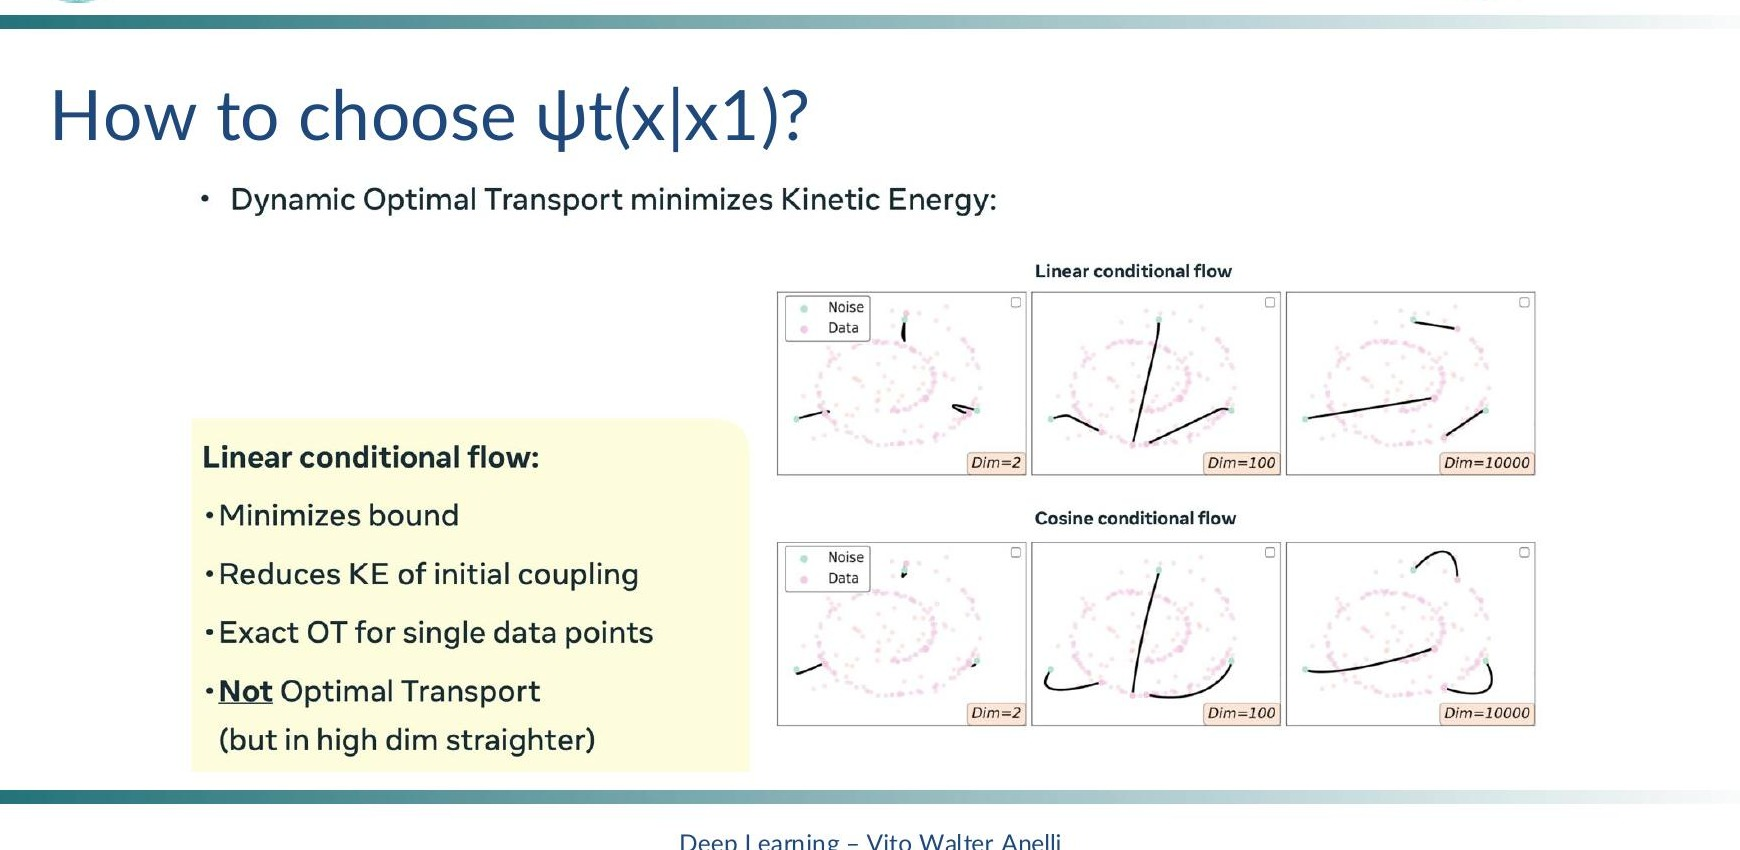
\includegraphics[width=0.88\linewidth]{figures/cf16_linear_vs_cosine.jpg}
  \caption{Confronto tra il flusso condizionale lineare (riga superiore)
           e il flusso condizionale cosinusoidale (riga inferiore) al
           crescere della dimensione ($d=2$, $d=100$, $d=10000$).
           In alta dimensione, le traiettorie lineari si raddrizzano
           sensibilmente, avvicinandosi al trasporto ottimale.}
  \label{fig:fm-linear-vs-cosine}
\end{figure}

\subsection{Flow Matching con Optimal Transport Condizionale}
\label{subsec:fm-cot}

Con la scelta lineare, la perdita CFM diventa:
\begin{align}
  \mathcal{L}_{\mathrm{CFM}}(\theta)
  &= \mathbb{E}\,D\!\left(u_t^\theta(X_t),\; u_t(X_t \mid X_1)\right) \notag\\
  &= \mathbb{E}\left\|u_t^\theta(X_t) - (X_1 - X_0)\right\|^2,
\end{align}
dove $X_t = (1-t)X_0 + tX_1$ e il coupling $(X_0, X_1) \sim \pi_{0,1}$
può essere scelto arbitrariamente (indipendente o strutturato).

%------------------------------------------------------------
\section{Traiettorie Affini e Percorsi Gaussiani}
\label{sec:fm-affine-gaussian}

\subsection{Traiettorie Affini}
\label{subsec:fm-affine}

Una famiglia generale di flussi condizionali è data dai
\textbf{percorsi affini}:
\begin{equation}
  \psi_t(x \mid x_1) = \alpha_t\,x_1 + \sigma_t\,x,
\end{equation}
con $\alpha_0 = 0$, $\alpha_1 = 1$, $\sigma_0 = 1$, $\sigma_1 = 0$
(o varianti con $\sigma_1 \approx 0$ per evitare singolarità).
La velocità corrispondente è:
\begin{equation}
  u_t(x) = \mathbb{E}\!\left[\dot\alpha_t X_1 + \dot\sigma_t X_0 \mid X_t = x\right].
\end{equation}

In questa forma, la velocità ammette tre \textbf{parametrizzazioni
equivalenti}:
\begin{description}
  \item[Predizione di velocità] $u_t(x) = \mathbb{E}[\dot\alpha_t X_1 + \dot\sigma_t X_0 \mid X_t = x]$
  \item[Predizione della sorgente $x_0$] (singolare a $t=0$):
    $u_t(x) = a_t\,x + b_t\,\mathbb{E}[X_0 \mid X_t = x]$
  \item[Predizione del target $x_1$] (singolare a $t=1$):
    $u_t(x) = c_t\,\mathbb{E}[X_1 \mid X_t = x] + d_t$
\end{description}

\subsection{Percorsi Gaussiani e Connessione con la Diffusione}
\label{subsec:fm-gaussian-paths}

Quando la distribuzione sorgente è gaussiana ($p = \mathcal{N}(0, I)$)
e il coupling è indipendente ($\pi_{0,1} = p \cdot q$), i percorsi
affini inducono distribuzioni condizionali gaussiane:
\begin{equation}
  p_{t|1}(x \mid x_1) = \mathcal{N}\!\left(\alpha_t x_1,\; \sigma_t^2 I\right).
\end{equation}
In questo caso, le tre parametrizzazioni della velocità si collegano
direttamente alle formulazioni standard dei modelli di diffusione:

\begin{center}
\begin{tabular}{ll}
  \toprule
  \textbf{Parametrizzazione} & \textbf{Corrispondente nei modelli di diffusione} \\
  \midrule
  Predizione sorgente $x_0$ & Predizione del rumore $\varepsilon$ (\emph{noise prediction}) \\
                             & Probability Flow ODE \\
  Predizione target $x_1$   & Predizione $x_1$ (\emph{denoiser}), $x_1$-prediction \\
  \bottomrule
\end{tabular}
\end{center}

I modelli di diffusione deterministici (es.\ DDIM) sono quindi un caso
speciale di Flow Matching con percorsi Gaussiani, distribuzione sorgente
gaussiana standard, e coupling indipendente \citep{song2020ddim}.

\begin{figure}[H]
  \centering
  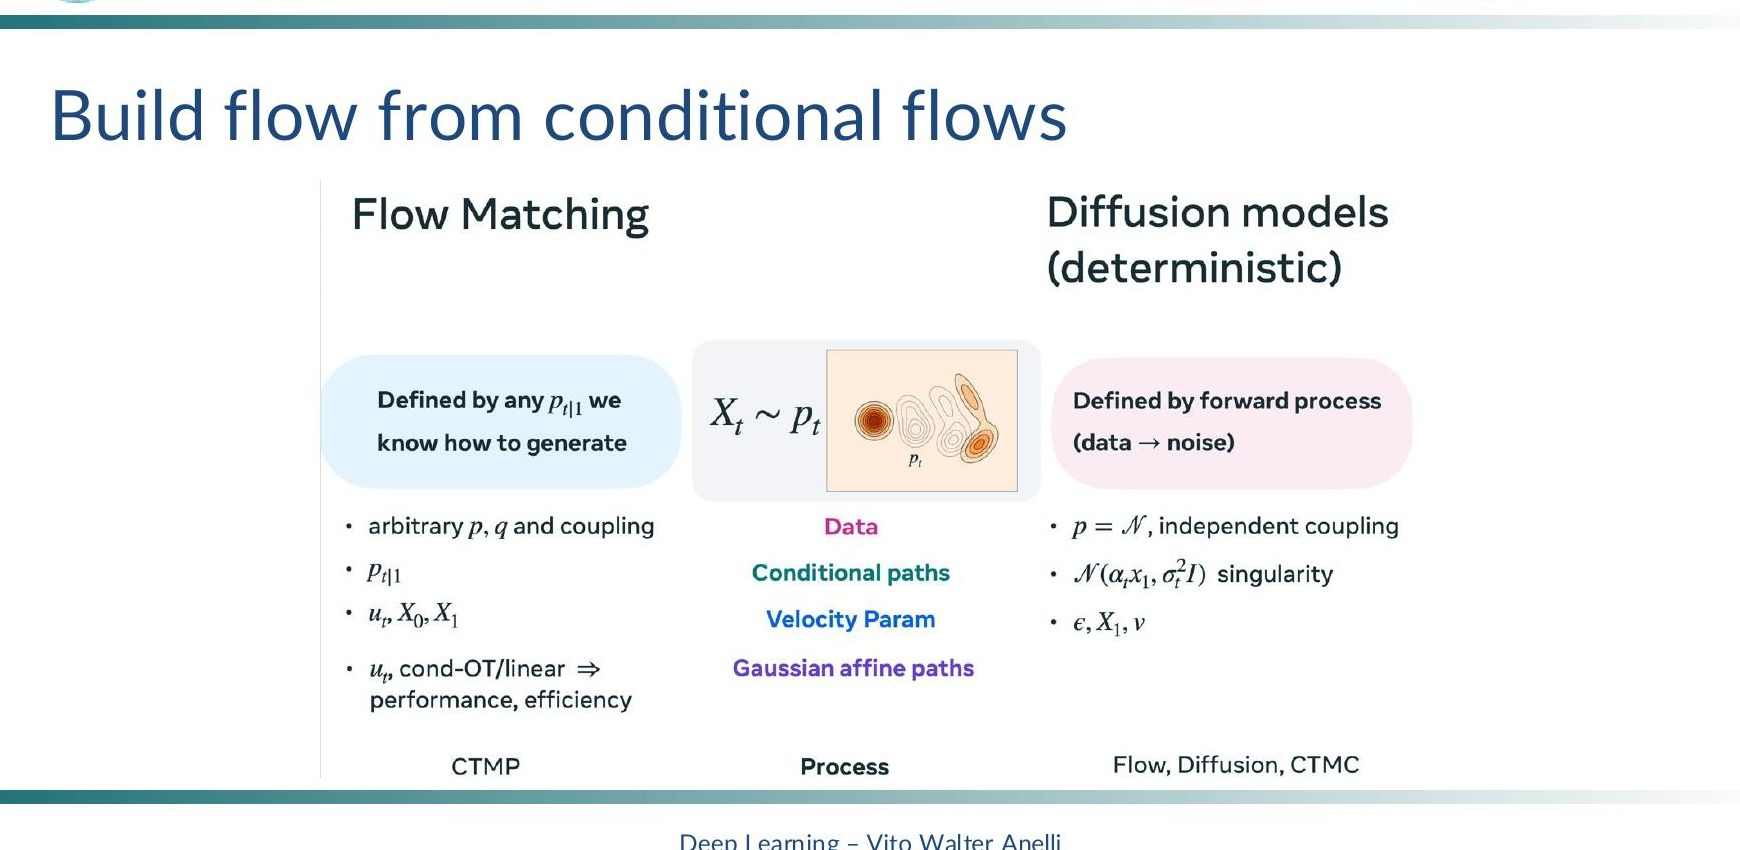
\includegraphics[width=0.82\linewidth]{figures/cf16_fm_vs_diffusion.jpg}
  \caption{Confronto tra Flow Matching e modelli di diffusione deterministici.
           Entrambi operano su processi a tempo continuo, ma si distinguono
           per la scelta del processo condizionale, del coupling e della
           parametrizzazione del campo vettoriale.}
  \label{fig:fm-vs-diffusion}
\end{figure}

%------------------------------------------------------------
\section{Reflow: Raddrizzamento delle Traiettorie}
\label{sec:fm-reflow}

\subsection{Motivazione}
\label{subsec:fm-reflow-motivation}

Anche con il flusso condizionale lineare, le traiettorie integrate
del modello addestrato possono risultare \textbf{curve} (non rettilinee),
perché la rete impara una media ponderata di direzioni che si incrociano.
Traiettorie curve richiedono più step di integrazione per essere
approssimate accuratamente con un solutore numerico, aumentando il costo
di campionamento.

Il \textbf{Reflow} \citep{liu2022flow} è una tecnica che permette di
raddrizzare iterativamente le traiettorie:

\begin{enumerate}
  \item Si inizializza con il flusso lineare standard (traiettorie rette
        ma con incroci durante il training).
  \item Si integra il modello corrente per ottenere coppie $(X_0, \hat X_1)$
        con $\hat X_1 = \text{ODE-solve}(u_t^\theta, X_0)$.
  \item Si riaddestra un nuovo modello FM su queste coppie
        $(\hat X_1, X_0)$, eliminando gli incroci e raddrizzando
        le traiettorie.
\end{enumerate}

\begin{figure}[H]
  \centering
  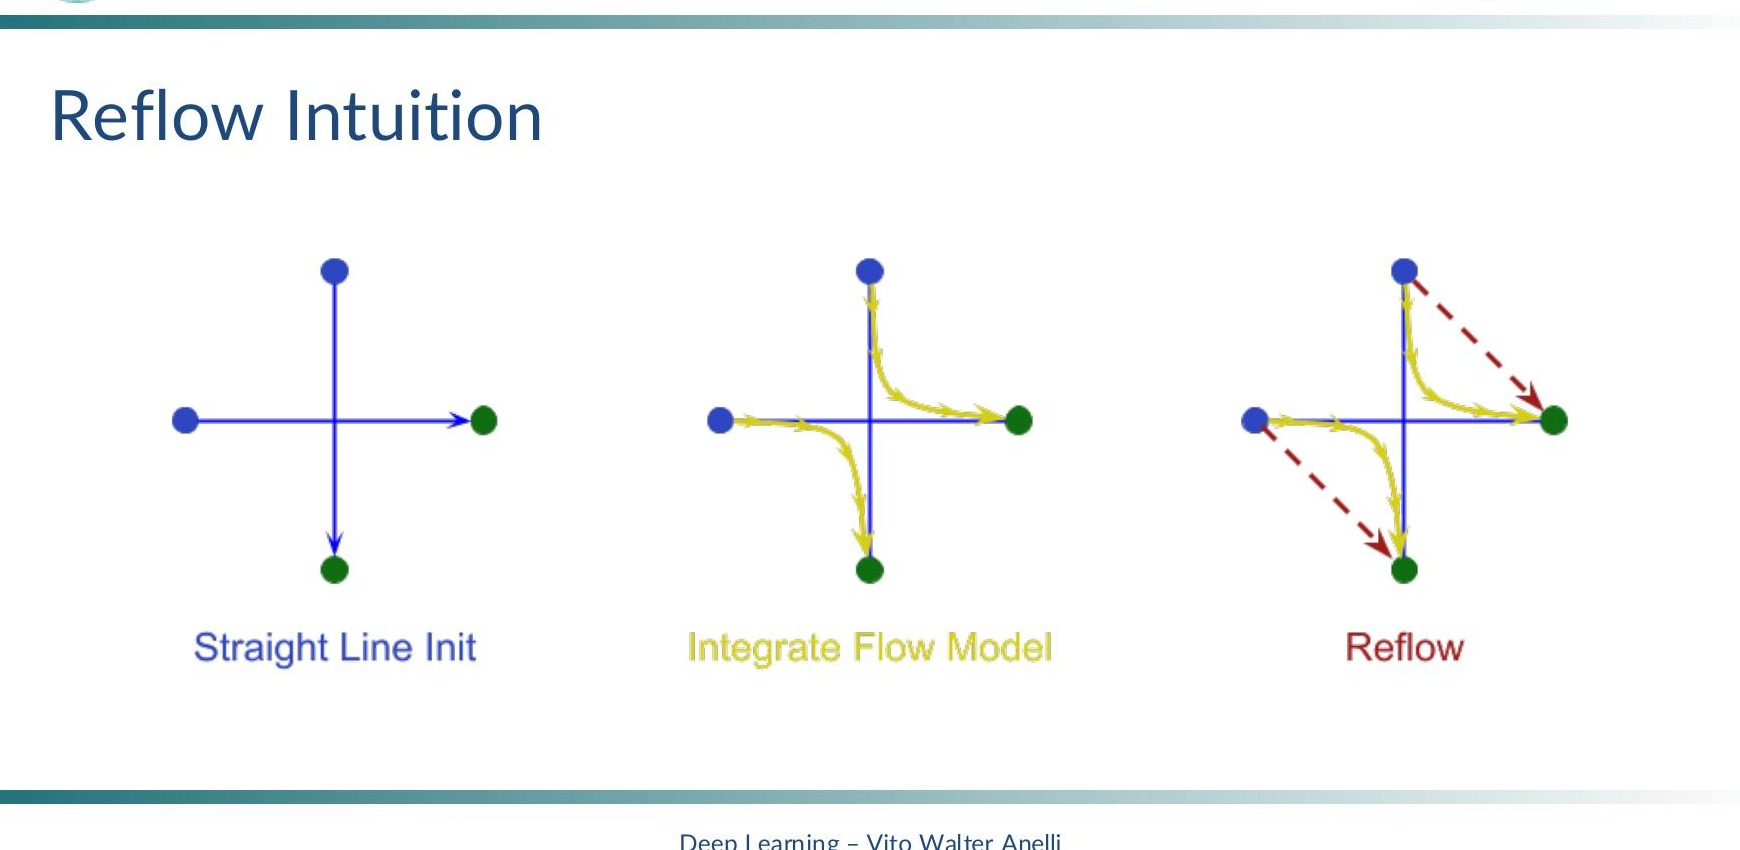
\includegraphics[width=0.85\linewidth]{figures/cf16_reflow_intuition.jpg}
  \caption{Intuizione del Reflow. \textbf{Sinistra}: traiettorie rette ma
           con incroci (initialization lineare). \textbf{Centro}: integrazione
           del modello corrente — le traiettorie si curvano attorno agli
           incroci. \textbf{Destra}: dopo il Reflow, le traiettorie si
           raddrizzano (linee tratteggiate rosse) grazie all'eliminazione
           degli incroci.}
  \label{fig:fm-reflow-intuition}
\end{figure}

\subsection{Effetti del Reflow}
\label{subsec:fm-reflow-effects}

Dopo il Reflow, le traiettorie risultano più rettilinee ma anche più
\textbf{curve globalmente}, a causa della riconfigurazione del campo
vettoriale per evitare incroci. La qualità dei campioni generati rimane
comparabile all'originale, ma l'integrazione può ora essere approssimata
con un minor numero di step (anche un unico step per modelli
sufficientemente reflowed).

%------------------------------------------------------------
\section{Flow Matching Condizionato}
\label{sec:fm-conditioning}

\subsection{Modelli Generativi Condizionali}
\label{subsec:fm-conditional-models}

Nella pratica, si desidera spesso campionare dalla distribuzione condizionale
$q(x_1 \mid y)$, dove $y$ è una condizione (es.\ una caption testuale,
un'etichetta di classe, o un'immagine di riferimento). Si modella un
campo di velocità condizionale:

\begin{align}
  p_{t \mid Y}(x \mid y) &=
    \mathbb{E}_{X_1}\!\left[p_{t|1}(x \mid X_1) \mid Y = y\right], \\
  u_t(x \mid y) &=
    \mathbb{E}\!\left[u_t(X_t \mid X_1) \mid X_t = x,\; Y = y\right].
\end{align}

La perdita di addestramento diventa:
\begin{equation}
  \mathcal{L}_{\mathrm{CFM}}(\theta) =
  \mathbb{E}_{t,\,(X_0, X_1, Y)\sim\pi_{0,1,Y}}\!
  \left\|u_t(X_t \mid X_1) - u_t^\theta(X_t \mid Y)\right\|^2,
\end{equation}
dove la stessa rete $u_t^\theta(x \mid y) : [0,1] \times \mathbb{R}^d \times \mathbb{R}^k \to \mathbb{R}^d$
è addestrata su tutte le condizioni simultaneamente.

\subsection{Guidance per Flow Matching}
\label{subsec:fm-guidance}

Analogamente alla diffusione, esistono due strategie di \emph{guidance}
per orientare il campionamento verso la distribuzione condizionale:

\paragraph{Classifier Guidance.}
Dato un modello incondizionato $u_t(x)$ e un classificatore
$p_{Y|t}(y \mid x)$ addestrato su campioni rumorosi, il campo guidato è:
\begin{equation}
  \tilde{u}_t(x \mid y) = u_t(x) + w\,b_t\,\nabla_x \log p_{Y|t}(y \mid x),
\end{equation}
dove $b_t$ è un fattore di scala che dipende dal percorso Gaussiano e
$w > 0$ è l'intensità della guidance.

\paragraph{Classifier-Free Guidance (CFG).}
Addestrando la stessa rete su condizioni con e senza etichetta
(dropout della condizione durante il training), il campo guidato diventa:
\begin{equation}
  \tilde{u}_t(x \mid y) = (1 - w)\,u_t(x) + w\,u_t(x \mid y).
  \label{eq:fm-cfg}
\end{equation}
Per $w = 1$ si ottiene il modello condizionato puro; per $w > 1$ si
amplifica la condizione a scapito della diversità
\citep{ho2022cfg,bishop2024}.

%------------------------------------------------------------
\section{Multimodal Diffusion Transformers (MMDiT)}
\label{sec:mmdit}

\subsection{Diffusion Transformer (DiT)}
\label{subsec:mmdit-dit}

Il \textbf{Diffusion Transformer} (DiT) \citep{peebles2023dit} è
un'architettura che sostituisce la classica U-Net nei modelli di diffusione
latente con un Transformer puro. I dati rumorosi nel spazio latente
($32 \times 32 \times 4$) vengono suddivisi in patch e proiettati in
token; il timestep $t$ e l'etichetta $y$ vengono iniettati tramite
il meccanismo \textbf{adaLN-Zero} (\emph{adaptive Layer Normalization}):
\begin{equation}
  h \leftarrow \bigl(\mathbf{1} + \gamma_1\bigr)\,\mathrm{LayerNorm}(h) + \beta_1,
\end{equation}
dove $\gamma_1$ e $\beta_1$ sono scalate e traslazioni prodotte da un
MLP che prende in input l'embedding del timestep e dell'etichetta.
Il residuo di attenzione viene modulato da un fattore $\alpha_1$
inizializzato a zero, garantendo che il blocco si riduca all'identità
a inizio training.

\subsection{Multi-Modal Diffusion Transformer (MMDiT)}
\label{subsec:mmdit-mmdit}

Il \textbf{MMDiT} estende il DiT al caso multimodale, consentendo
l'interazione bidirezionale tra sequenze di token eterogenee (es.\
token testuali e token immagine). La chiave architettonica è il
meccanismo di \textbf{Joint Attention}:

\begin{enumerate}
  \item I token di testo e di immagine vengono proiettati separatamente
        in spazi QKV tramite pesi lineari \emph{distinti}.
  \item Le sequenze di Q, K, V vengono concatenate lungo la dimensione
        della sequenza e si calcola un'unica attenzione congiunta.
  \item I risultati vengono separati e restituiti ai rispettivi stream
        (testo e immagine), ciascuno modulato indipendentemente.
\end{enumerate}

\begin{figure}[H]
  \centering
  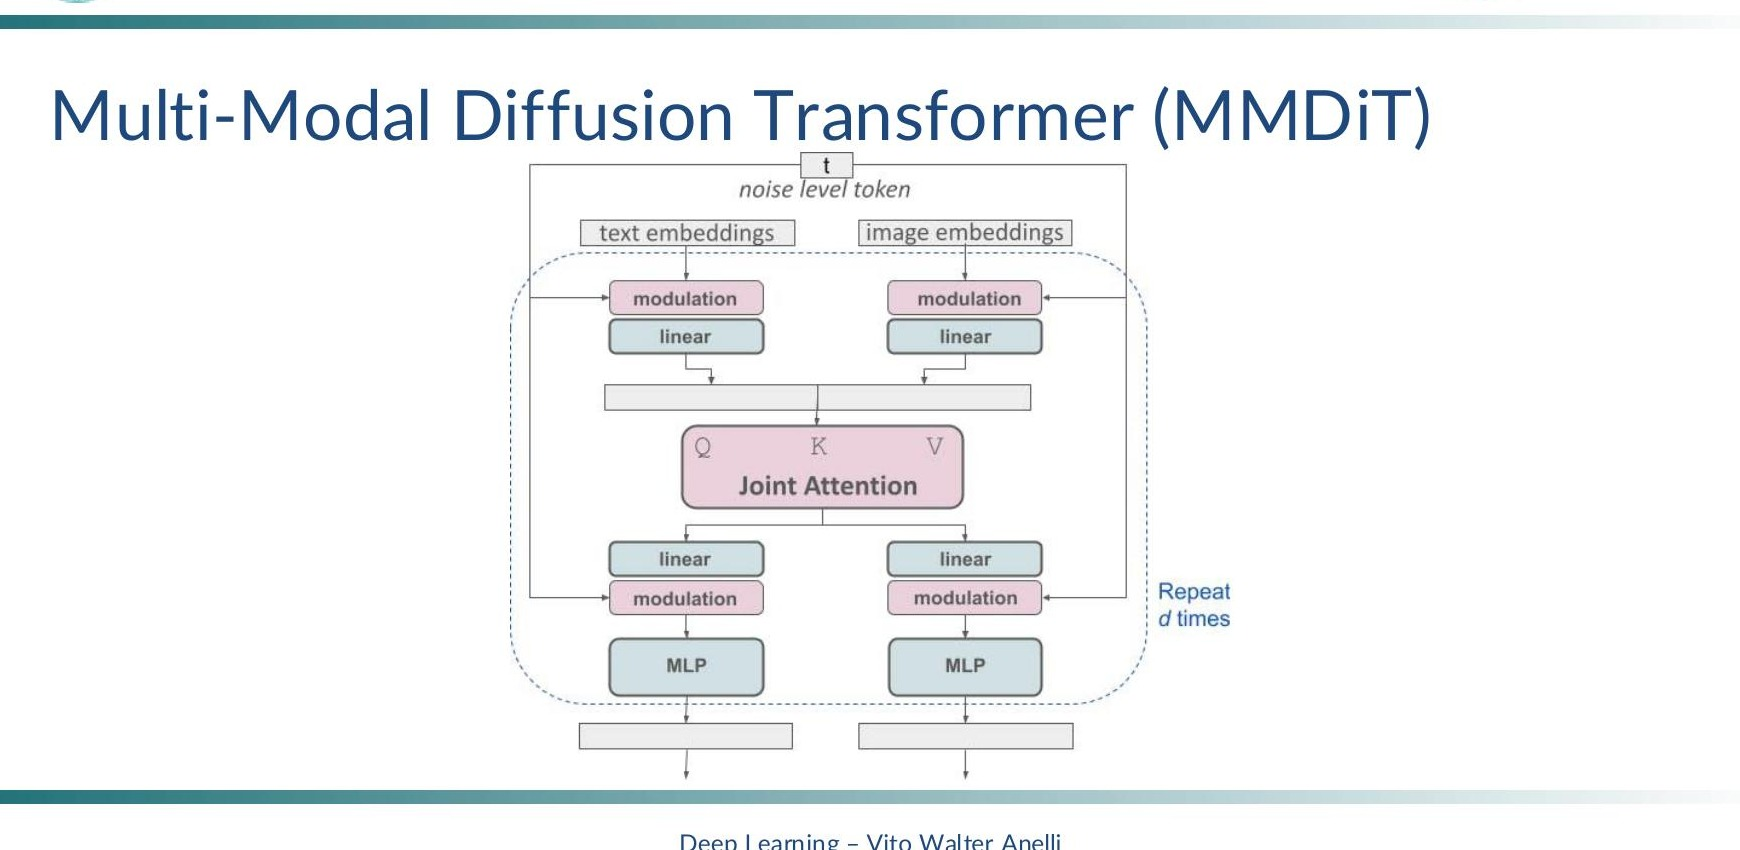
\includegraphics[width=0.65\linewidth]{figures/cf16_mmdit_block.jpg}
  \caption{Un blocco MM-DiT. I due stream (testo a sinistra, immagine a
           destra) condividono il meccanismo di attenzione congiunta
           (Joint Attention) ma mantengono pesi lineari e modulation MLP
           separati. Il token di livello di rumore $t$ modula entrambi
           gli stream tramite il meccanismo adaLN.}
  \label{fig:mmdit-block}
\end{figure}

%------------------------------------------------------------
\section{Stable Diffusion 3}
\label{sec:sd3}

\subsection{Architettura Complessiva}
\label{subsec:sd3-architecture}

\textbf{Stable Diffusion 3} (SD3) \citep{esser2024sd3} è un modello
testo-immagine allo stato dell'arte che combina Flow Matching con
l'architettura MMDiT. I componenti principali sono:

\begin{description}
  \item[\textbf{Text Encoders}] Tre encoder testuali in parallelo:
    CLIP-G/14, CLIP-L/14 e T5 XXL. I token contestuali di CLIP-L e
    CLIP-G (77+77 token) vengono concatenati lungo i canali e proiettati
    in 4096 dimensioni come condizione testuale $c$. I pooled embedding
    di CLIP-G/14 vengono sommati all'embedding del timestep per formare
    il vettore di condizione globale $y$.
  \item[\textbf{Latent VAE}] Il \emph{Noised Latent} è ottenuto
    codificando l'immagine in uno spazio latente tramite un VAE
    (risoluzione ridotta), aggiungendo rumore gaussiano, e poi
    patchificando il risultato tramite una proiezione lineare.
  \item[\textbf{Positional Embedding}] Embedding posizionale 2D sommato
    ai token immagine prima dei blocchi MM-DiT.
  \item[\textbf{MM-DiT Blocks}] Una sequenza di $d$ blocchi MM-DiT
    che elaborano congiuntamente token testuali e immagine, aggiornati
    entrambi a ogni layer.
  \item[\textbf{Output}] Dopo gli $d$ blocchi, un layer di
    modulazione e una proiezione lineare producono il campo di velocità
    stimato; il risultato viene de-patchificato per ricostruire la
    predizione nel spazio latente.
\end{description}

\begin{figure}[H]
  \centering
  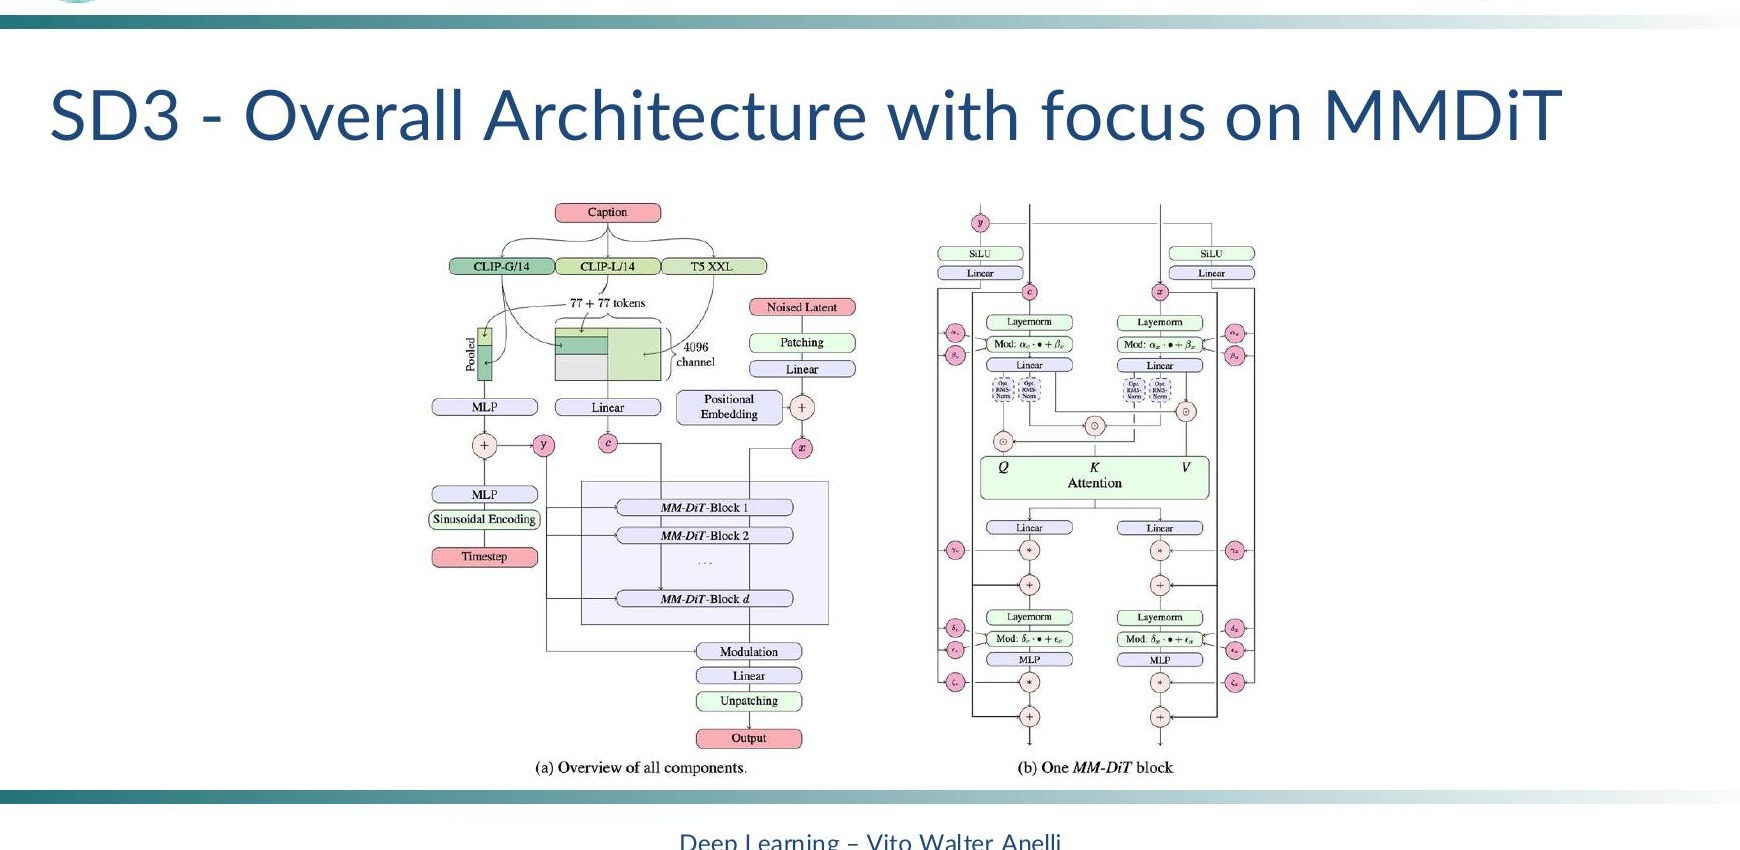
\includegraphics[width=0.88\linewidth]{figures/cf16_sd3_architecture.jpg}
  \caption{Architettura completa di Stable Diffusion 3. Il percorso
           superiore elabora la caption testuale tramite tre encoder
           (CLIP-G/14, CLIP-L/14, T5 XXL) e produce gli embedding
           contestuali $c$ e globali $y$. Il percorso inferiore processa
           il latent rumoroso con patchify e positional embedding. Entrambi
           i flussi di informazione vengono elaborati congiuntamente
           all'interno dei blocchi MM-DiT, iterati $d$ volte.}
  \label{fig:sd3-architecture}
\end{figure}

\subsection{Il Ruolo di T5 in SD3}
\label{subsec:sd3-t5}

\textbf{T5} (\emph{Text-To-Text Transfer Transformer}) \citep{raffel2020t5}
è un modello encoder-decoder basato su Transformer che inquadra qualsiasi
compito NLP come un problema testo-a-testo. In SD3, viene utilizzata la
variante \textbf{T5 XXL} come encoder testuale, per la sua capacità di
rappresentare testi con semantica ricca e dipendenze a lunga distanza.

Le caratteristiche architetturali principali di T5 sono:

\begin{itemize}
  \item \textbf{Relative Positional Embeddings} con bias scalare aggiunto
        alla matrice di attenzione: $A_{ij} \leftarrow A_{ij} + b(i-j)$.
  \item \textbf{Pre-LayerNorm}: la normalizzazione è applicata
        \emph{all'ingresso} di ogni blocco (non all'uscita come in BERT),
        con una variante ``scale-only'' (RMSNorm senza bias).
  \item \textbf{Pre-training con Span Corruption}: porzioni contigue di
        token vengono mascherate e il modello viene addestrato a
        ricostruirle, un'estensione del Masked Language Model a span
        interi (anziché token singoli come in BERT).
  \item \textbf{Attenzione Causale con Prefisso} (\emph{Prefix LM}):
        la sequenza di input usa attenzione bidirezionale, mentre la
        sequenza di output usa attenzione causale (unidirezionale).
\end{itemize}

T5 è stato pre-addestrato sul dataset \textbf{C4} (\emph{Colossal Clean
Crawled Corpus}) con un obiettivo di denoising, e poi fine-tuned su
molteplici task (GLUE, SuperGLUE, SQuAD, WMT) usando un approccio
multi-task unificato. In SD3, solo l'encoder T5 viene utilizzato: i
suoi output token vengono concatenati con quelli di CLIP e usati come
condizione testuale nel MMDiT.

\subsection{Formazione del Modello e Scelte di Design}
\label{subsec:sd3-training}

Le principali scelte di design che distinguono SD3 dai predecessori sono:

\paragraph{Flow Matching con OT condizionale.}
SD3 utilizza la formulazione lineare di Flow Matching ($X_t = (1-t)X_0 + tX_1$)
con coupling indipendente, che produce traiettorie quasi rettilinee in
alta dimensione e permette un campionamento efficiente con pochi step.

\paragraph{Architettura MMDiT scalabile.}
Il design con stream separati per testo e immagine, ma attenzione
congiunta, permette di scalare i pesi del modello in modo efficiente:
si può raddoppiare la profondità del modello senza modificare le
interfacce tra le componenti.

\paragraph{Tre encoder testuali complementari.}
CLIP-G e CLIP-L catturano relazioni semantiche visivo-testuali globali;
T5 XXL cattura strutture linguistiche complesse e descrizioni testuali
dettagliate. La combinazione migliora la fedeltà al testo rispetto all'uso
di un solo encoder.

%------------------------------------------------------------
\section{Procedura di Addestramento e Campionamento}
\label{sec:fm-training-sampling}

\subsection{Procedura di Training}
\label{subsec:fm-training}

L'addestramento di un modello Flow Matching segue i seguenti passi ad
ogni iterazione:

\begin{enumerate}
  \item \textbf{Campionare} coppie $(X_0, X_1)$ dalla distribuzione
        sorgente $p$ e dalla distribuzione target $q$ (eventualmente
        con un coupling strutturato $\pi_{0,1}$).
  \item \textbf{Campionare} un tempo $t \sim \mathrm{Uniform}[0,1]$.
  \item \textbf{Calcolare} la posizione interpolata
        $X_t = (1-t)X_0 + tX_1$ — dove il punto si troverebbe se si
        muovesse a velocità costante da $X_0$ a $X_1$.
  \item \textbf{Calcolare} la velocità target $\dot X_t = X_1 - X_0$
        (costante lungo la traiettoria lineare).
  \item \textbf{Aggiornare} i parametri $\theta$ minimizzando
        $\|u_t^\theta(X_t) - (X_1 - X_0)\|^2$. La rete impara la
        ``media'' delle velocità di tutti i punti che passano per
        $X_t$ al tempo $t$.
\end{enumerate}

L'approccio è \textbf{simulation-free}: a differenza dei modelli di
diffusione che richiedono l'integrazione dell'SDE durante il training,
il Flow Matching non richiede mai di simulare la traiettoria.

\subsection{Campionamento}
\label{subsec:fm-sampling}

Per generare un campione:
\begin{enumerate}
  \item Campionare $X_0 \sim \mathcal{N}(0, I)$.
  \item Integrare l'ODE $\frac{d}{dt}X_t = u_t^\theta(X_t)$
        da $t=0$ a $t=1$ con un solutore numerico
        (es.\ metodo di Eulero, metodo del punto medio o Runge-Kutta 4).
  \item Restituire $X_1$ come campione dalla distribuzione target.
\end{enumerate}

Il metodo del \textbf{punto medio} (Heun/RK2) è particolarmente adatto
in quanto offre un buon compromesso tra accuratezza e costo computazionale.
Con traiettorie sufficientemente rettilinee (ottenute con OT condizionale
o Reflow), anche un singolo step di Eulero può produrre campioni di
buona qualità.

%------------------------------------------------------------
\section{Connessioni con Altri Modelli Generativi}
\label{sec:fm-connections}

\begin{table}[H]
  \centering
  \caption{Confronto tra Flow Matching, modelli di diffusione e approcci
           diretti. FM = Flow Matching, DDPM = Denoising Diffusion
           Probabilistic Model, DDIM = Denoising Diffusion Implicit Model,
           OT-CFM = Conditional OT Flow Matching.}
  \label{tab:fm-comparison}
  \small
  \adjustbox{max width=\linewidth}{%
  \begin{tabular}{lccccc}
    \toprule
    \textbf{Aspetto}
      & \textbf{FM/OT-CFM}
      & \textbf{DDPM}
      & \textbf{DDIM}
      & \textbf{GAN}
      & \textbf{VAE} \\
    \midrule
    Simulation-free training & \checkmark & \checkmark & \checkmark & \checkmark & \checkmark \\
    Traiettorie rettilinee   & \checkmark & $\times$  & $\times$  & n/a & n/a \\
    Verosimiglianza esatta   & \checkmark & $\times$  & $\times$  & $\times$ & $\approx$ \\
    Campionamento efficiente & \checkmark & $\times$  & $\approx$ & \checkmark & \checkmark \\
    Coupling arbitrario      & \checkmark & $\times$  & $\times$  & $\times$ & $\times$ \\
    Stabilità di training    & alta & alta & alta & bassa & alta \\
    \bottomrule
  \end{tabular}%
  }
\end{table}

In sintesi, il Flow Matching unifica e generalizza i modelli di diffusione
deterministici (DDIM) come caso speciale con percorsi Gaussiani e coupling
indipendente, mentre aggiunge la flessibilità di scegliere coupling
arbitrari (es.\ mini-batch OT) e percorsi non Gaussiani, con il vantaggio
computazionale di traiettorie tendenzialmente più rettilinee e quindi
campionamento più rapido \citep{lipman2022flow,liu2022flow,albergo2022building,bishop2024}.
